\documentclass{tufte-handout}

\title{Course Syllabus\\
	Philosophy of Sport} %\thanks{Inspired by Edward~R. Tufte!}}

\author[Craig T. Carley]{Professor Craig Carley}

\date{Phoenix College: Spring 2014} % without \date command, current date is supplied

%\geometry{showframe} % display margins for debugging page layout

\usepackage{graphicx} % allow embedded images
  \setkeys{Gin}{width=\linewidth,totalheight=\textheight,keepaspectratio}
  \graphicspath{{graphics/}} % set of paths to search for images
\usepackage{amsmath}  % extended mathematics
\usepackage{booktabs} % book-quality tables
\usepackage{units}    % non-stacked fractions and better unit spacing
\usepackage{multicol} % multiple column layout facilities
\usepackage{lipsum}   % filler text
\usepackage{fancyvrb} % extended verbatim environments
  \fvset{fontsize=\normalsize}% default font size for fancy-verbatim environments
\usepackage{colortbl}
\usepackage{hyperref}

% Standardize command font styles and environments
\newcommand{\doccmd}[1]{\texttt{\textbackslash#1}}% command name -- adds backslash automatically
\newcommand{\docopt}[1]{\ensuremath{\langle}\textrm{\textit{#1}}\ensuremath{\rangle}}% optional command argument
\newcommand{\docarg}[1]{\textrm{\textit{#1}}}% (required) command argument
\newcommand{\docenv}[1]{\textsf{#1}}% environment name
\newcommand{\docpkg}[1]{\texttt{#1}}% package name
\newcommand{\doccls}[1]{\texttt{#1}}% document class name
\newcommand{\docclsopt}[1]{\texttt{#1}}% document class option name
\newenvironment{docspec}{\begin{quote}\noindent}{\end{quote}}% command specification environment

\begin{document}


\maketitle% this prints the handout title, author, and date

%------------------------------------ DEFINE COLORS -------------------
\definecolor{blue}{HTML}{ADD8E6}
\definecolor{lightblue}{HTML}{D4E1E6}
\definecolor{darkblue}{HTML}{172285}
\definecolor{red}{HTML}{E69AA2}
\definecolor{lightred}{HTML}{E6C4C6}
\definecolor{brown}{HTML}{665322}

\marginnote{\textsc{MCCCD Course Description} General consideration of sport in its philosophical dimensions. Possible topics include the Zen of sport, strategy and competition, sport, practice, and play, and cheating versus fair play.}

\begin{marginfigure}%
  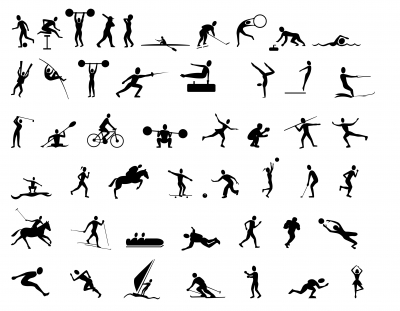
\includegraphics[width=\linewidth]{../assets/SPORTS.jpg}
  \caption{Symbols of various sports.}
  \label{fig:marginfig}
\end{marginfigure}

\begin{abstract}
\noindent
\color{brown} "Hockey is a sport for white men. Basketball is a sport for black men. Golf is a sport for white men dressed like black pimps."
\begin{flushright}
---Tiger Woods
\end{flushright}

\noindent
"Serious sport has nothing to do with fair play. It is bound up with hatred, jealousy, boastfulness, disregard of all rules and sadistic pleasure in witnessing violence. In other words, it is war minus the shooting."
\begin{flushright}
---George Orwell
\end{flushright}

\noindent
"I'd just as soon play tennis with the net down."
\begin{flushright}
---Robert Frost
\end{flushright}

\end{abstract}

%\printclassoptions
\marginnote{\vspace{0.2in}\\
\color{darkblue} 
Since I do spend alot of time in Canvas, contacting me \textit{via} your Canvas Inbox is my preferred method of connecting with students.}

\section{Instructor Information}\label{sec:instructor}
\begin{center}
\begin{tabular}{ll}
  \rowcolor{blue}
  \textsc{name} & Craig Carley\\
  \rowcolor{lightblue}
  \textsc{dept} & Liberal Arts\\
  \rowcolor{blue}
  \textsc{building} & A-137 \\
  \rowcolor{lightblue}
  \textsc{phone} & 602.285.7651 \\
  \rowcolor{blue}
  \textsc{email} & \url{mailto:craig.carley@phoenixcollege.edu}\\
  \rowcolor{lightblue}
  \textsc{smc} & 480.250.2971 \\
  \rowcolor{blue}
  \textsc{web} & \url{http://www.phoenixcollege.edu/}\\
  \rowcolor{lightblue}
  \textsc{canvas} & \url{https://learn.maricopa.edu/login}\\
  \rowcolor{blue}
  \textsc{hours} & TR 10:30a - 11:30a \\
  \rowcolor{lightblue}
  \textsc{ } & and by appointment \\
 \end{tabular}
\end{center}

\marginnote{\textsc{Course Competencies:} (1.) Distinguish philosophy from other forms of inquiry. (2.) Distinguish sport from other forms of activity. (3.) Contrast and criticize the views of Plato and Aristotle on sport. (4.) Summarize and critique competing positions on the mind-body problem. (5.) Analyze the concepts of practice, competition, and individual vs. team sports. (6.) Differentiate between and evaluate knowledge paradigms and apply to various sporting scenarios. (7.) Interpret and critique the aesthetic qualities of sport and play. (8.) Contrast different normative ethical approaches. (9.) Appraise and evaluate various ethical issues associated with sports. (10.) Critique the role of sport within its social and political context.}


\section{Course Information}\label{sec:course}
% 21321 REL243	A110 	In Person 	01/14/2014- 05/09/2014 	Tu,Th 	11:30AM- 12:45PM 	
% 21704 REL243	A106 	Hybrid 		01/14/2014- 05/09/2014 	Tu 		1:00PM- 2:30PM
% 21702 PHI251	C201 	In Person 	01/13/2014- 05/09/2014 	M,W 	10:00AM- 10:50AM 	


\begin{center}
\begin{tabular}{lll}
  \rowcolor{red}
  \textsc{name} & Philosophy of Sport\\
  \rowcolor{lightred}
  \textsc{number} & PHI251\\
  \rowcolor{red}
  \textsc{campus} & Phoenix College | Main Campus\\
  \rowcolor{lightred}
  \textsc{section} & 21702 \\
  \rowcolor{red}
  \textsc{type} & Hybrid \\ 
  \rowcolor{lightred}
  \textsc{semester} & 2014 - Spring\\
  \rowcolor{red}
  \textsc{dates} & 14 Jan - 9 May\\
  \rowcolor{lightred}
  \textsc{days} & Mon \Verb|&| Wed\\ 
  \rowcolor{red}
  \textsc{times} & 10:00a - 10:50p \\ 
  \rowcolor{lightred}
  \textsc{Location} & C201\\ 
\end{tabular}
\end{center}

\newpage

\section{Course Materials}

\begin{marginfigure}%
  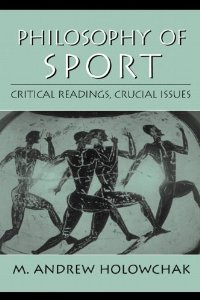
\includegraphics[width=\linewidth]{../assets/phil-of-sport.jpg}
  \caption{Required Textbook}
  \label{fig:marginfig}
\end{marginfigure}

\subsection{Required Texts}
Although I am not opposed to students sharing a textbook, it is better if you have your own textbook. You can rent the textbook or buy it and then resell it at the end of the semester if you wish to offset some of the expense. The book we will be using, \textit{Philosophy of Sport: Critical Readings, Crucial Issues} (ISBN: \href{http://www.amazon.com/Philosophy-Sport-Critical-Readings-Crucial/dp/0130941220}{\color{darkblue}0130941220}), is pictured to the left.\sidenote{\color{brown}Holowchak, M. Andrew. \textit{Philosophy of Sport: Critical Readings, Crucial Issues}. Pearson, 2002. Print.}

The success of this class depends on your active and enthusiastic involvement. You will be expected to engage your colleagues in intelligent discourse; this will presuppose your having read the assignments. So please, read the text and the assignments carefully.

\subsection{From the Back Cover}
This anthology draws from philosophical, sociological, and psychological literature as it explores the philosophy of sport. The collected essays treat diverse and contemporary issues and inquire into questions such as: What is sport? Are female athletes of the same rank as men? Are many sports too violent? Should certain drugs be banned? Each essay is accompanied by questions and exercises that invite critical discussion.

\subsection{Canvas}
All your work will be submitted and graded in Canvas\sidenote{\href{https://learn.maricopa.edu}{\color{darkblue}https://learn.maricopa.edu}}, so please familiarize yourself with how it works and where things are located in it. If you have questions, please ask---chances are one of your colleagues has similiar concerns.

All tests, writing assignments, handouts, and readings that are not in the textbook will be made available on Canvas.

\section{Course Requirements}
\subsection{Final Grade Calculation}
There will be a total of 1000 points available for this course. The following table reflects how final letter grades will be calculated (the numeric values represent percentages):

\begin{marginfigure}%
  
\includegraphics[width=\linewidth]{../assets/lettergrades.jpg}
  \caption{Final Grades based on Percentages of Total Points}
  \label{fig:marginfig}
\end{marginfigure}

\begin{fullwidth}

\begin{center}
  \begin{tabular}{  c | c  c | c  c }
    \hline
    \rowcolor{Grey}
    Grade & Low PCT. & High PCT. & Low PTS. & High PTS.\\ \hline \hline
    \rowcolor{BurntOrange}
    A & 90.0 & 100.0 & 900 & 1000 \\ \hline
    \rowcolor{Yellow}
    B & 80.0 & 89.9 & 800 & 899 \\ \hline
    \rowcolor{SkyBlue}
    C & 70.0 & 79.9 & 700 & 799 \\ \hline
    \rowcolor{LimeGreen}
    D & 60.0 & 69.9 & 600 & 699\\ \hline
    \rowcolor{Red}
    F & 0.0  & 59.9 & 0 & 599\\     
    \hline
  \end{tabular}
\end{center}
\end{fullwidth}

\subsection{Assessments and Distributions}

\begin{fullwidth}

The final grade is a composite of a variety of components. The relative weights of these components are given in the following table:

\vspace{0.2in}

\begin{center}
	\begin{tabular}{  l  c  r  }
	  \hline
	  \rowcolor{blue}
	  \textbf{Component} & \textbf{Points} & \textbf{Relative Weight} \\ \hline \hline
	  \rowcolor{lightblue}
	  4-Tests (lowest score will be dropped) & 300 & 30 percent \\ \hline
	  \rowcolor{blue}
	  4-Papers (lowest score will be dropped) & 300 & 30 percent \\ \hline
	  \rowcolor{lightblue}
	  10-Homework and Group Work  & 100 & 10 percent \\ \hline
	  \rowcolor{blue}
	  2-Audio-Visual Presentations & 200 & 20 percent \\ \hline
	  \rowcolor{lightblue}
	  Attendance and Participation & 100 & 10 percent \\ \hline
	  \rowcolor{blue}
	  TOTAL & 1000 & 100 percent \\ 
	  \hline
	\end{tabular}
\end{center}

\subsection{Description of Components}
\begin{center}
\textsc{Tests} \\
\end{center}
There will be four tests each worth 100 points. The lowest test score will be dropped from the final grade calculation---hence there will be a maximum of 300 total test points. These test will consist of: 20-30 multiple choice and fill-in-the-blank questions (60 points) and 2 essay questions (40 points). These tests will be delivered \textit{via} Canvas. You will have 90 minutes to complete each test. All tests must be completed by the due date.
\begin{center}
\textsl{Sample Questions}
\end{center}
\begin{enumerate}
	\item In \textit{Is Sport Unique? A Question of Definability}, S.K. Wertz draws primarily on the work of which of the following philosophers in his argument against an essentialist understanding of sport.
	\begin{enumerate}
		\item Quine
		\item Collingwood
		\item Wittgenstein
		\item Galvin
	\end{enumerate}
	\item In \textit{Paternalism, Drugs, and the Nature of Sport}, W.M. Brown presents his view on the use of performance-enhancing drugs (PEDs). 
	\begin{enumerate}
		\item Under what conditions would Brown advocate the use of PEDs and under what conditions would he not advocate their use? (7 points)
		\item Explain Brown's reasoning with respect to the above conditions. (7 points)
		\item Explain how a critic of Brown's view might attempt to show his position to be untenable. (6 points)
	\end{enumerate}
\end{enumerate}

\begin{center}
\textsc{Papers} \\
\end{center}
Four papers will be assigned over the course of the semester. Each paper will be worth 100 points. Again, the paper with the lowest score will be dropped from the final grade calculation---bring the maximum paper point total to 300. These papers should be 3-5 pages in length, use proper spelling and grammar, and submitted in Canvas by the due date. No hardcopies or scanned hand-written papers will be accepted. Each paper will be written in response to a prompt which I will provide when the assignment is released (approximately 2 weeks before the due date). More details on these assignments and a grading rubric will be provided on Canvas. So, please stay current and check Canvas regularly.

\begin{center}
\textsl{Sample Paper Prompt}
\end{center}
Was there a political, educational, or social agenda for the establishment of the modern Olympic Games? If so, who were the individuals involved and how did these political, educational, or social issues manifest themselves?

\begin{center}
\textsc{Homework and Group Work}
\end{center}
There will be 10 assignments in this category---each worth 10 points. The nature of the assignments will vary in form and requirements, so instructions will be provided when the assignment is given. Typical assignments: a one page reflection paper on an assigned video, completion of an article survey, examining a case study and answering a few follow-up questions, etc.

\end{fullwidth}

\vspace{0.15in}

\begin{center}
\textsc{Audio-Visual Presentation}
\end{center}

There will be two A/V presentations required. Each will be worth 100 points. You should design your presentations around issues which we have encountered throughout the semester. Since we will not have time to present all student presentations in a live classroom setting, I'm asking you to create a video which everyone can watch at their leisure. 

Your presentation should be approximately 6-12 minutes in length. You should introduce your audience to your topic, highlight at least three major talking points, and present your concluding remarks.

Your presentation will not be peer-reviewed, however I hope you will watch the presentations of your collegues and offer some encouraging remarks. See the course schedule below for the due dates of each presentation.

\begin{marginfigure}%
  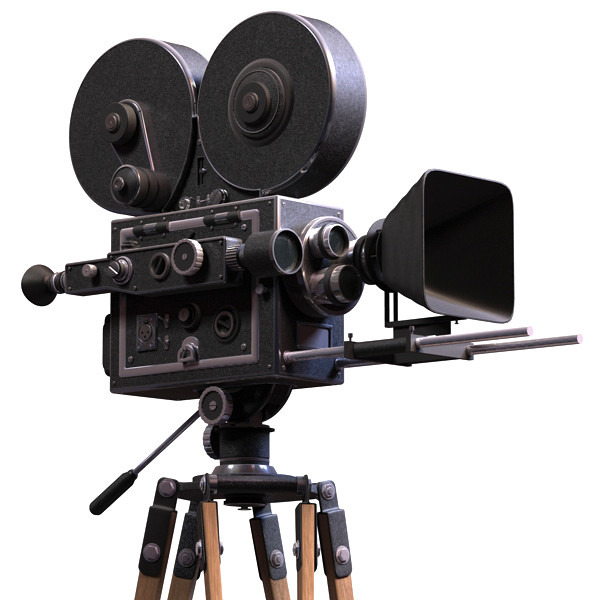
\includegraphics[width=\linewidth]{../assets/moviecamera.jpg}
  \caption{Don't worry about making a high quality HD video. A standard camera phone or digital camera is sufficient. You might also screencast your desktop $\ldots$ we will talk more about this later.}
  \label{fig:marginfig}
\end{marginfigure}

More details on this assignment and a grading rubric will be provided on Canvas.

\begin{center}
\textsc{Attendance and Class Participation}
\end{center}
Your presence in class and online will determine your participation points. Excessive absenses will result in a reduction of points for the period in question. Failure to participate on the online discussion boards may also result in a reduction of participation points.

Although I will do my best to make the class an entertaining and significant experience, your participation is required. Please ask questions, make comments, offer criticisms, and state your opinions and views. Although my classes are loosely structured, I don't want the discussion time to become a free-for-all, so some respect and consideration is required. Also, please address each other in a respectful manner and only criticize the position, never the individual. If I find excessive chatter has a disruptive influence on the class, I will ask for silence. If this persists, I will ask the individuals responsible for the disruption to leave the class.

\section{Class Policies and Responsibilities}
\subsection {Attendance, Withdrawals and Tardiness}

\begin{marginfigure}%
  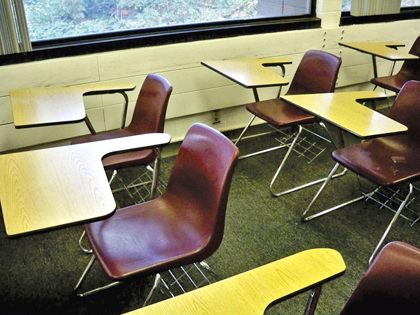
\includegraphics[width=\linewidth]{../assets/emptydesks.jpg}
  \caption{Come to class $\ldots$ it's boring when you don't show-up.}
  \label{fig:marginfig}
  \vspace{0.3in}
\end{marginfigure}

\begin{center}
\textsc{Attendance Policy}
\end{center}

I will take attendance regularly and reserve the right to withdraw you for excessive unexcused absences. In the case of lecture style courses, missing more than four hours of classroom time constitutes excessive absences. In the case of Blackboard style courses failure to log in on a weekly basis constitutes excessive absences. It is ultimately your responsibility to withdraw from the course should you find that necessary. If you do wish to withdraw for any reason, please email me to make arrangements. Do not simply stop attending class. If you are absent, it is your responsibility to obtain missing notes from a classmate.

\begin{marginfigure}%
  
\includegraphics[width=\linewidth]{../assets/raisinghands.jpg}
  \caption{Raise your hand. Be polite and don't talk over your collegues.}
  \label{fig:marginfig}
\end{marginfigure}

\begin{center}
\textsc{Withdrawal Procedures}
\end{center}

A student may officially withdraw from specific courses in the following ways: Through the 7th week, a student may initiate an official withdrawal from any course by completing the withdrawal process on-line using the student self-service system or by submitting a course withdrawal form to the Admissions and Records Office/Office of Student Enrollment Services in accordance with the published deadlines. A grade of W (withdrawn, passing not computed in the grade point average) will be assigned. After the 7th week , a student must initiate a withdrawal request with the faculty member. If, after consultation with the student, the faculty member approves the request, a grade of W (withdrawn, passing---not computed in the grade point average) or Y (withdrawn,
failing---computed in the grade point average as a failing grade) will be assigned. If the request is not approved, the student will remain in the course.

\vspace{0.7in}

\begin{center}
\textsc{Tardiness Policies}
\end{center}

Please arrive on time to class. Arriving late or departing early is disruptive to the class and is discourteous to all members of the class. Arriving 15 minutes late or departing 15 minutes early will constitute an unexcused absence. If you wish to appeal such an unexcused absence, you must present your reasons to me in-person on the day that it occurs.

\begin{center}
\textsc{Academic Misconduct}
\end{center}

\begin{marginfigure}%
  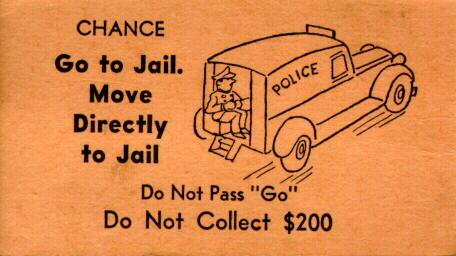
\includegraphics[width=\linewidth]{../assets/gotojail.jpg}
  \caption{Don't copy and paste. Be sure to cite your sources.}
  \label{fig:marginfig}
\end{marginfigure}

Academic misconduct includes, among other things, plagiarism, cheating on exams or papers, and disruption of class. At a minimum, you will receive a score of zero on any exam, quiz, or paper involving academic misconduct. Depending on the seriousness of the offense, I may also reduce a final grade, remove the student from class, and/or refer the student for disciplinary action.

If you feel lost or insecure about the course material, making an appointment with me is a much better option than resorting to cheating or plagiarism. I sincerely want to help you learn the material and prepare you for the future. Cheating prevents you from learning, prevents me from helping, and ultimately could stand in the way of your future success.

\marginnote{For a complete list of academic policies---e.g., attendance, grading, instructional grievance process, withdrawal, academic misconduct---which govern the Maricopa Community College District refer to: \href{http://www.maricopa.edu/publicstewardship/governance/adminregs/students/2_3.php}{\color{darkblue}MCCCD Policy Manual}}

\begin{center}
\textsc{Late Work}
\end{center}
No late work will be accepted unless a documented family/medical emergency, religious obligations, or college-sanctioned activity conflicts. I am happy to accommodate such events, but I must be told as far in advance as possible.

In the case where the student misses an in-class test or quiz, please see me to make arrangements as soon as possible.

\begin{fullwidth}

\vspace{0.1in}

\begin{center}
\textsc{Extra Credit}
\end{center}
At this time there is no provision being made for extra credit work.

\vspace{0.1in}

\begin{center}
\textsc{Returning Graded Work}
\end{center}
I strive to return graded work within one week from its submission. You should always retain a copy of what you submit and the graded work I return. If you do not collect your graded work by the last day of the semester, it may be discarded. You may leave me a self-addressed, stamped envelope if you wish to have your work returned to you by mail.

\vspace{0.1in}

\begin{center}
\textsc{Grade Disputes}
\end{center}
I will carefully and thoughtfully grade all of your assignments. If you disagree with a grade on any assignment or assessment, you must submit a written statement of the reasons for your disagreement within one week of receiving the grade.

\vspace{0.2in}

\begin{center}
\textsc{Electronic Devices}
\end{center}
As a courtesy to the class (includingd me), all electronic devices should be set to silent mode during class. If you are expecting an urgent call, please use non-audible settings and leave the classroom before answering. Please do not electronically record the class without my prior permission.

\end{fullwidth}

\section{Resource for Students}
\subsection{Disability Accommodations}
I am more than happy to make reasonable accommodations for disability-related limitations. Please see me to discuss any special needs you might have. If you have, or believe you have, a disability and would benefit from any accommodations, you may wish to self identify by contacting Disability Services at 602.285.7477 are on-line at: \href
{http://www.phoenixcollege.edu/student-resources/disability}{\color{darkblue}PC Student Resources Disability Page}

\subsection{Counseling Services}
The counseling department provides free and confidential assistance with life skills, career planning and crisis intervention. The counseling offices may be reached at 602.285.7392 or on-line at: \href
{http://www.phoenixcollege.edu/student-resources/support-services/counseling}{\color{darkblue}PC Student Resources Counseling Page}

\begin{marginfigure}%
  
\includegraphics[width=\linewidth]{../assets/success.jpg}
  \caption{Many resources and services are available to help you succeed.}
  \label{fig:marginfig}
\end{marginfigure}

\subsection{Success Center}
The Success Center provides services, resources and programs to support students at Phoenix College so they can develop skills essential for successful learning. The Success Center is located on the second floor (Room 228) of the B-building. Call 602.285.7486 or visit on-line at: \href
{http://www.phoenixcollege.edu/student-resources/success-center}{\color{darkblue}PC Student Resources Success Center Page}

\section{Compliance with Policies}

\marginnote{\textsc{Disclaimer:} This syllabus is a tentative plan for the course and may be altered, orally or in writing, at my discretion. Course content may also vary from this syllabus to meet the needs of this particular class. It is your responsibility to keep abreast of changes to the syllabus.}

Every student is expected to know and comply with all current published policies, rules and regulations as printed.


\section{Class Schedule and Readings}
There are nine chapters in our textbook and we will be covering all of them. This works out to about one chapter every two weeks. However, the first and last chapters will be allotted only one week. For each chapter there will be a quiz and a discussion board required. The due dates for all assignments will be made available as the assignments are posted.

\vspace{0.1in}

\begin{fullwidth}

\begin{center}
\begin {tabular} {l l l}
	\hline
	\rowcolor{lightblue}
	\textsc{Week} & \textsc{Topic} & \textsc{Assignments and Readings} \\
	\hline
	\rowcolor{blue}
	Jan 13 & Introduction &  Carley, \textit{Philosophical Tools and Argument} \\
	\rowcolor{lightblue}
	Jan 20 & Games, Play, and Humanity & Huizinga (1), \textit{Homo Ludens} \\
	\rowcolor{lightblue}
		& &	Loy (2), \textit{The Nature of Sport} \\
	\rowcolor{blue}
	Jan 27 & Conceptual Analysis of Sport & Suits (3), \textit{Tricky Triad} \\
	\rowcolor{blue}
		& & Meier (4), \textit{Triad Trickery} \\
	\rowcolor{lightblue}
	Feb 03 & Conceptual Analysis of Sport & Wertz (8) \textit{Is Sport Unique?} \\
	\rowcolor{lightblue}
		& & \textbf{Test 1 and Paper 1 due \textsl{via} Canvas by Feb 9$^{th}$} \\
	\rowcolor{blue}
	Feb 10 & Sport in Antiquity &   Mechikoff, \textit{Ancient Civilizations: Greece} \\
	\rowcolor{lightblue}
	Feb 17 & Sport in Modernity &   Mechikoff, \textit {Modern Olympic Games: 1896-1936} \\
	\rowcolor{lightblue}
		& & Mechikoff, \textit {Modern Olympic Games: 1948-1988} \\
	\rowcolor{blue}
	Feb 24 & Sport and Aesthetics & Kaelin (9) \textit{The Well-Played Game} \\
	\rowcolor{blue}
		& & Best (10), \textit{The Aesthetic in Sport} \\
	\rowcolor{blue}
		& & Cordner (12), \textit{Differences between Sport and Art} \\
	\rowcolor{lightblue}
	Mar 03 & Postmodern Society and Sport & Morgan (41), \textit{Sport in the Larger Scheme} \\
	\rowcolor{lightblue}
		& & Arnold (42), \textit{Democracy, Education, and Sport} \\
	\rowcolor{lightblue}
		& & Morgan (43), \textit{Sport and the Making of National Identities} \\
	\rowcolor{blue}
		& & \textbf{Test 2 and Paper 2 due \textsl{via} Canvas by March 9$^{th}$} \\
	\rowcolor{blue}
	Mar 10 & \textbf{SPRING BREAK} &  \\
	\rowcolor{lightblue}
	Mar 17 & Performance Enhancing Drugs & Brown (24), \textit{Paternalism, Drugs and Nature of Sport} \\
	\rowcolor{lightblue}
		& & Gardener (25), \textit{On PED and the Unfair Advantage Argument} \\
	\rowcolor{lightblue}
		& & \textbf{A-V Presentation 1 due \textsl{via} Canvas by March 23$^{rd}$} \\
	\rowcolor{blue}
	Mar 24 & Performance Enhancing Drugs &  Holowchak (26), \textit{Aretism: Taking a Shot at Steroids} \\
	\rowcolor{blue}
		& & Parry (22) \textit{Violence and Aggression in Sport}\\
	\rowcolor{lightblue}
	Mar 31 & Sportsmanship and Violence & Arnold (13), \textit{Three Approaches to Sportsmanship} \\
	\rowcolor{lightblue}
		& & Simon (14), \textit{Sportsmanship and Fairness in Pursuit of Victory} \\
	\rowcolor{blue}
	Apr 07 & Sportsmanship and Cheating &  \textbf{Paper 3 and Test 3 due \textsl{via} Canvas by March 23$^{rd}$}\\
	\rowcolor{lightblue}
	Apr 14 & Sports and Aggression & Holowchak (40), \textit{Aggression, Gender, and Sport} \\
	\rowcolor{blue}
	Apr 21 & Sports, Sex and Gender Issues & Boxill (33), \textit{Title IX and Gender Equity} \\
	\rowcolor{blue}
		& & Francis (35), \textit{Title IX: Equality for Women in Sports} \\
	\rowcolor{blue}
		& & \textbf{A-V Presentation 2 due \textsl{via} Canvas by Apr 27$^{th}$} \\
	\rowcolor{lightblue}
	Apr 28 & Sexism and Racism in Sport & Postow (32), \textit{Women and Masculine Sport} \\
	\rowcolor{lightblue}
		& & Kidd (34), \textit{The Men's Cultural Centre} \\
	\rowcolor{lightblue}
		& & Burfoot (36), \textit{White Men Can't Run} \\
	\rowcolor{lightblue}
		& & Mosley (37). \textit{Racial Differences in Sport} \\
	\rowcolor{blue}
		May 05 & & \textbf{Test 4 and Paper 4 due \textsl{via} Canvas by May 9$^{th}$}   \\
	\hline
\end {tabular}
\end{center}

\end{fullwidth}

\bibliography{sample-handout}
\bibliographystyle{plainnat}

\end{document}
